\section{Sign of a number}
\subsection{Aim}
To check whether a number is positive or negative using bit manipulation

\subsection{Code}
\begin{lstlisting}
DATA SEGMENT
    num DW 0000H
    positives DB 'Positive', '$'
    negatives DB 'Negative', '$'
    zeros DB 'Zero', '$'   
DATA ENDS

CODE SEGMENT
ASSUME CS:CODE, DS:DATA  
START:
    MOV AX, DATA
    MOV DS, AX
    MOV AX, num
    SHR AX, 15 
    MOV BX, AX
    MOV AX, num
    NEG AX
    SHR AX, 15
    SUB AX, BX
    ADD AX, 1
    CMP AX, 2
    JE POSITIVE
    CMP AX, 1
    JE ZERO
    LEA DX, negatives
    MOV AH, 09H
    INT 21H
    JMP EXIT
POSITIVE:
    LEA DX, positives
    MOV AH, 09H
    INT 21H
    JMP EXIT
ZERO:
    LEA DX, zeros
    MOV AH, 09H
    INT 21H
EXIT:
    MOV AH, 4CH
    INT 21H
CODE ENDS
END START
\end{lstlisting}

\subsection{Output}
\begin{center}
	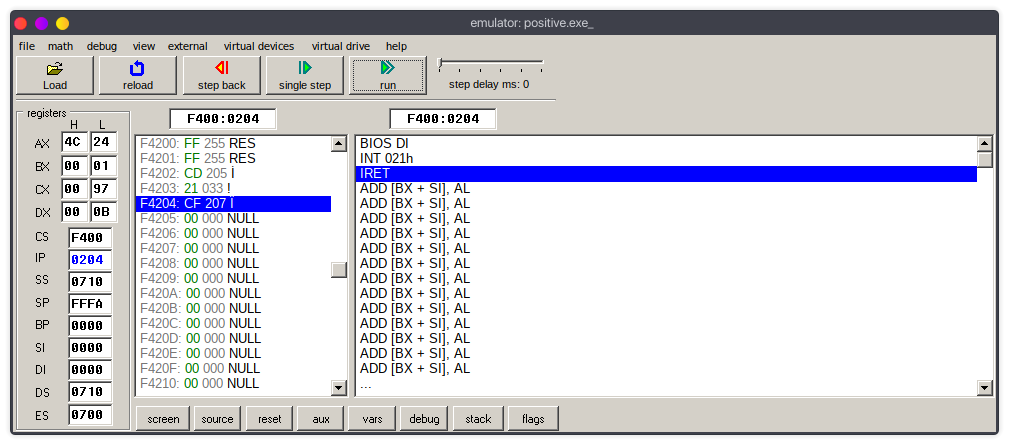
\includegraphics[width=0.90\textwidth]{img/p14/ss1.png}
	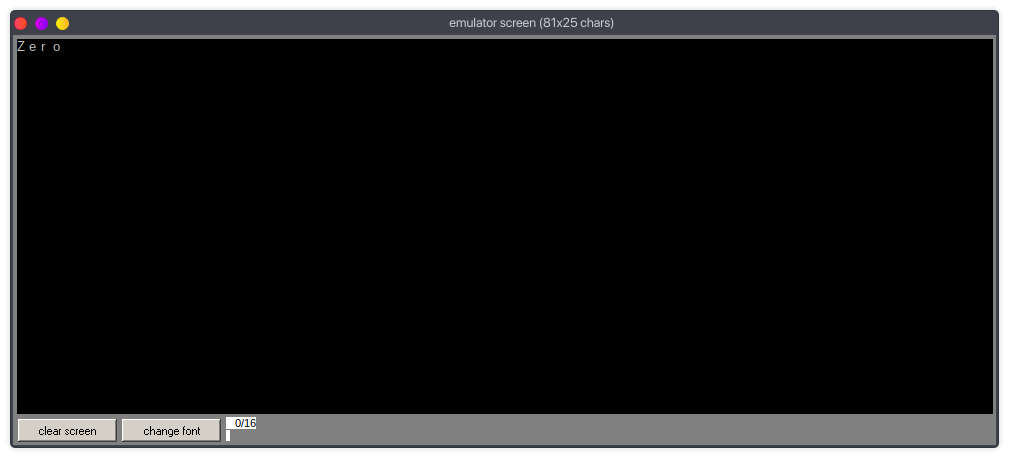
\includegraphics[width=0.90\textwidth]{img/p14/ss2.png}\\
	Output for 0000H\\

	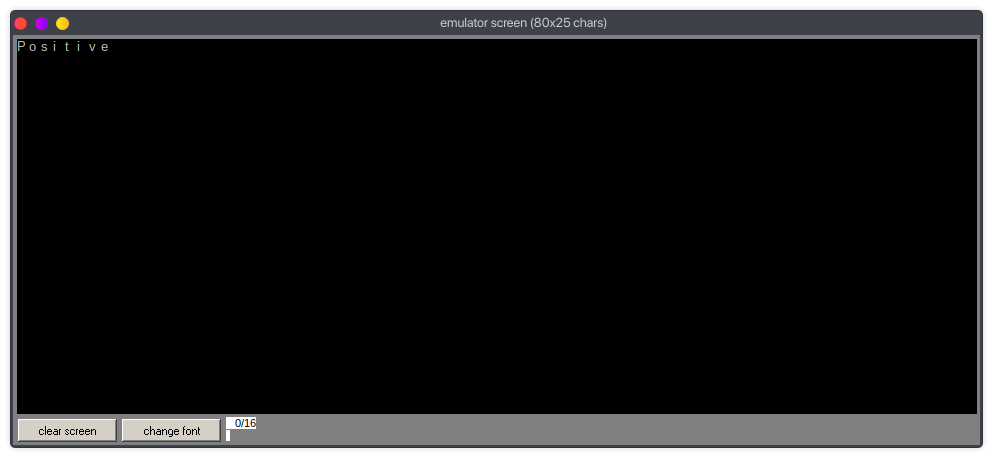
\includegraphics[width=0.90\textwidth]{img/p14/ss3.png}\\
	Output for 0001H\\

	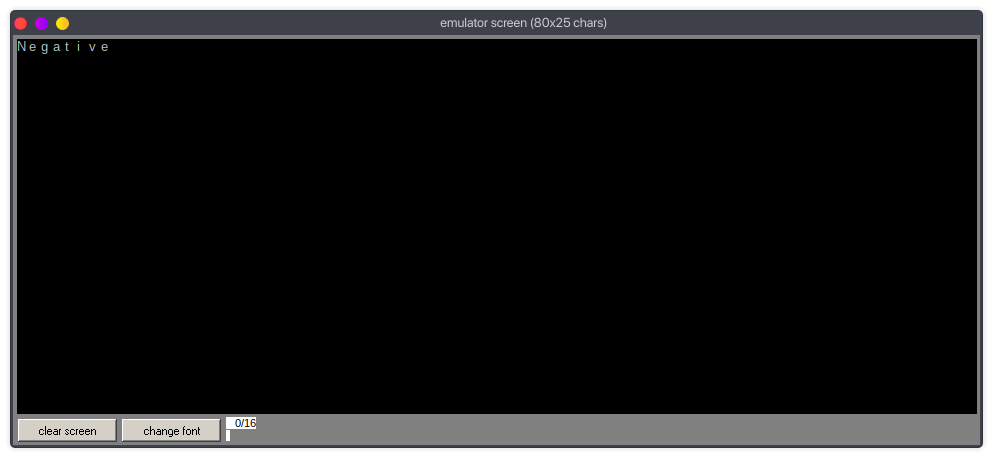
\includegraphics[width=0.90\textwidth]{img/p14/ss4.png}\\
	Output for -0001H
\end{center}

\subsection{Result}
Sign of an integer was found out using bit manipulation

